В информационный центр приходят клиенты через интервал времени $10\pm2$ минуты. Если все три имеющихся оператора заняты, клиенту отказывают в обслуживании. Операторы имеют разную производительность и могут обеспечивать обслуживание среднего запроса пользователя за $20\pm5$; $40\pm10$; $40\pm20$. Клиенты стремятся занять свободного оператора с максимальной производительностью. Полученные запросы сдаются в накопитель. Откуда выбираются на обработку. На первый компьютер запросы от 1 и 2-ого операторов, на второй – запросы от 3-его. Время обработки запросов первым и 2-м компьютером равны соответственно $15$ и $30$ мин.

Промоделировать процесс обработки 300 запросов.

\begin{figure}[h]
	\begin{center}
		{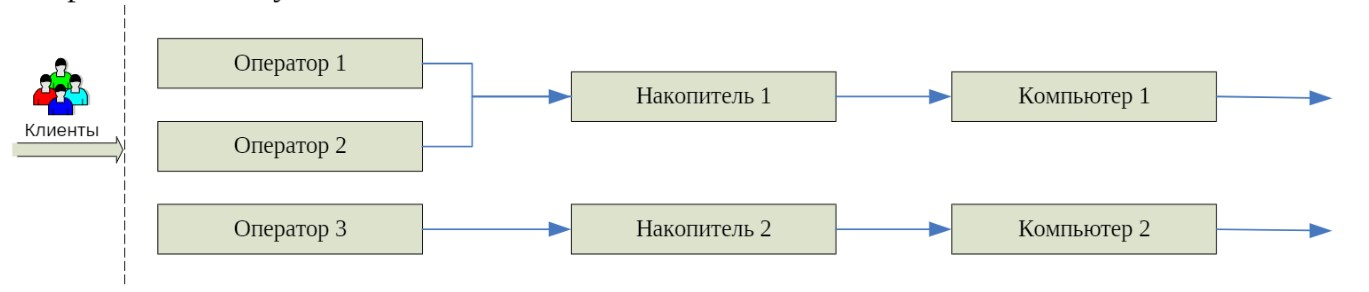
\includegraphics[scale=0.6]{task.jpg}
			\caption{Визуальное описание задания}
			\label{pic:1}}
	\end{center}
\end{figure}